\documentclass[12pt, twoside]{article}
\input{../preamble}

\fancyhead[LO]{La Scuola d'Italia / Dr.\ Huson / IB Math AA SL \\* 12 May 2026}
\fancyhead[RO]{\fbox{\begin{minipage}{4cm}\footnotesize First \& Last name:\\[0.5cm]\end{minipage}}}
\fancyfoot[C]{\thepage}

\pgfplotsset{compat=1.18}

\newcommand{\ticketTable}{%
\begin{center}
\renewcommand{\arraystretch}{1.45}
\begin{tabular}{|c|c|}
\hline
\shortstack{\textbf{Number of tickets}\\ \textbf{sold, }$n$}
&
\shortstack{\textbf{Number of}\\ \textbf{performances}}\\ \hline
$0<n\leq 200$ & $3$\\ \hline
$200<n\leq 400$ & $p$\\ \hline
$400<n\leq 600$ & $18$\\ \hline
$600<n\leq 800$ & $30$\\ \hline
\end{tabular}
\end{center}
}

\newcommand{\cumulativeGraph}{%
\begin{center}
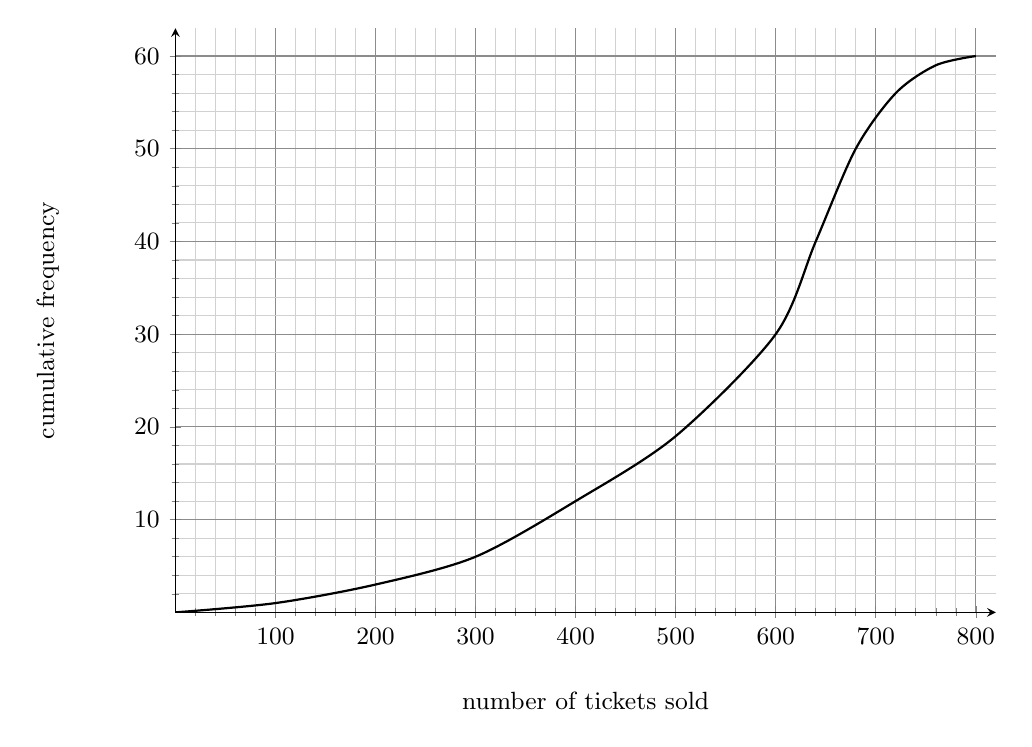
\begin{tikzpicture}
\begin{axis}[
  xlabel={number of tickets sold},
  ylabel={cumulative frequency},
  xmin=0, xmax=820,
  ymin=0, ymax=63,
  xtick={0,100,...,800},
  ytick={0,10,...,60},
  minor x tick num=4,
  minor y tick num=4,
  grid=both,
  major grid style={black!45},
  minor grid style={black!18},
  axis lines=middle,
  enlargelimits=false,
  width=12cm,
  height=9cm,
  tick label style={font=\small},
  label style={font=\small},
  xlabel style={at={(axis description cs:0.5,-0.12)}, anchor=north},
  ylabel style={at={(axis description cs:-0.13,0.5)}, anchor=south, rotate=90},
]
\addplot[smooth, thick, no markers] coordinates {
  (0,0)
  (100,1)
  (200,3)
  (300,6)
  (400,12)
  (500,19)
  (600,30)
  (640,40)
  (680,50)
  (720,56)
  (760,59)
  (800,60)
};
\end{axis}
\end{tikzpicture}
\end{center}
}

\newcommand{\boxPlot}{%
\begin{center}
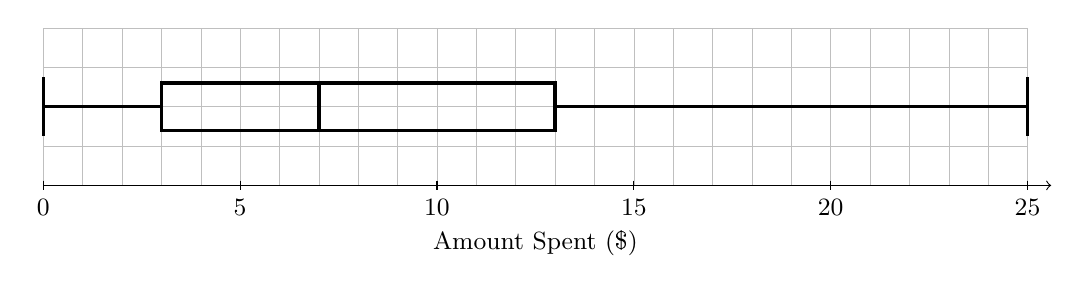
\begin{tikzpicture}[x=0.50cm,y=0.5cm]
  \draw[very thin, black!25, step=1] (0,0) grid (25,4);
  \draw[->] (0,0) -- (25.6,0);
  \foreach \x in {0,5,10,15,20,25}
    \draw (\x,0.12) -- (\x,-0.12) node[below, font=\small] {$\x$};

  \def\minv{0}
  \def\qone{3}
  \def\med{7}
  \def\qthree{13}
  \def\maxv{25}

  \draw[very thick] (\minv,2) -- (\qone,2);
  \draw[very thick] (\qthree,2) -- (\maxv,2);
  \draw[very thick] (\qone,1.4) rectangle (\qthree,2.6);
  \draw[very thick] (\med,1.4) -- (\med,2.6);
  \draw[very thick] (\minv,1.25) -- (\minv,2.75);
  \draw[very thick] (\maxv,1.25) -- (\maxv,2.75);

  \node[below, font=\small] at (12.5,-0.9) {Amount Spent (\$)};
\end{tikzpicture}
\end{center}
}

\begin{document}
\subsubsection*{11.17 Classwork: Cumulative Frequency and Normal Models}

Answer on lined paper. Problem 1 is no calculator. Problem 2 is calculator allowed.

\begin{enumerate}[itemsep=0.3cm]

%--- Problem 1: Cumulative frequency, sampling, box plot, and variance [17 marks] ---
%--- Source: AA SL 2023 Nov P1 TZ2 Q7 ---
\item[1.] \makebox[\linewidth][s]{[Maximum mark: 17]\hfill {\small AA SL 2023 Nov P1 TZ2 Q7}}

A ballet company performs \emph{The Nutcracker} every year. Last year
they gave a total of $60$ performances at their theatre which has a
maximum capacity of $800$. The number of tickets sold, $n$, at each
performance is shown in the following frequency table.

\ticketTable

\begin{enumerate}[itemsep=0.12cm]
  \item[(a)] \begin{enumerate}[itemsep=0.08cm]
    \item[(i)] Find the value of $p$. \hfill [1]
    \item[(ii)] Write down the modal class. \hfill [1]
  \end{enumerate}
\end{enumerate}

The following cumulative frequency diagram also displays these data.

\cumulativeGraph

Use the cumulative frequency curve to estimate

\begin{enumerate}[itemsep=0.12cm]
  \item[(b)] \begin{enumerate}[itemsep=0.08cm]
    \item[(i)] the median number of tickets sold; \hfill [1]
    \item[(ii)] the number of performances where at least $80\%$ of the
    tickets were sold. \hfill [3]
  \end{enumerate}
\end{enumerate}

\newpage

After a performance, the company decides to conduct a survey to obtain
feedback from the audience.

\begin{enumerate}[itemsep=0.12cm]
  \item[(c)] \begin{enumerate}[itemsep=0.08cm]
    \item[(i)] State one disadvantage of the company surveying only the
    first $5\%$ of the audience as they leave the theatre. \hfill [1]
    \item[(ii)] Describe briefly how the company could collect feedback
    from $5\%$ of the audience using the systematic sampling method.
    \hfill [2]
    \item[(iii)] State the sampling method which should be used if the
    survey is to be representative of the number of children and the
    number of adults in the audience. \hfill [1]
  \end{enumerate}
\end{enumerate}

Last year $36\,000$ tickets were sold to \emph{The Nutcracker}.

The following box and whisker diagram displays the amount spent by the
audience at the souvenir shop when they attended the performance.

\boxPlot

\begin{enumerate}[itemsep=0.12cm]
  \item[(d)] \begin{enumerate}[itemsep=0.08cm]
    \item[(i)] Estimate the number of people who spent between $\$3$ and
    $\$25$. \hfill [2]
    \item[(ii)] Half the audience spent less than $\$a$. Estimate the
    value of $a$. \hfill [1]
  \end{enumerate}
\end{enumerate}

This year the company will again give $60$ performances and expects to
sell $17$ additional tickets for each performance.

\begin{enumerate}[itemsep=0.12cm]
  \item[(e)] \begin{enumerate}[itemsep=0.08cm]
    \item[(i)] Calculate the mean number of tickets the company expects
    to sell this year for each performance. \hfill [3]
    \item[(ii)] State what effect, if any, this increase in ticket sales
    would have on the variance of the number of tickets sold for each
    performance. \hfill [1]
  \end{enumerate}
\end{enumerate}

\newpage

%--- Problem 2: Normal model followed by binomial and conditional probability [16 marks] ---
%--- Source: AA SL 2023 Nov P2 TZ1 Q9 ---
\item[2.] \makebox[\linewidth][s]{[Maximum mark: 16]\hfill {\small AA SL 2023 Nov P2 TZ1 Q9}}

A farmer is growing a field of rice plants. The height, $H$ cm, of each
plant can be modelled by a normal distribution with mean $\mu$ and
standard deviation $\sigma$.

It is known that
\[
P(H<82.4)=0.213
\qquad\text{and}\qquad
P(H>87.3)=0.409.
\]

\begin{enumerate}[itemsep=0.16cm]
  \item Find the probability that the height of a randomly selected plant
  is between $82.4$ cm and $87.3$ cm. \hfill [2]
  \item Find the value of $\mu$ and the value of $\sigma$. \hfill [5]
\end{enumerate}

The farmer measures $100$ randomly selected plants. Any plant with a
height greater than $87.3$ cm is considered ready to harvest. Heights of
plants are independent of each other.

\begin{enumerate}[itemsep=0.16cm]
  \item[(c)] \begin{enumerate}[itemsep=0.08cm]
    \item[(i)] Find the probability that exactly $32$ plants are ready to
    harvest. \hfill [2]
    \item[(ii)] Given that fewer than $44$ plants are ready to harvest,
    find the probability that exactly $32$ plants are ready to harvest.
    \hfill [4]
  \end{enumerate}
\end{enumerate}

In another field, the farmer is growing the same variety of rice, but is
using a different fertilizer. The heights of these plants, $F$ cm, are
normally distributed with mean $92.8$ and standard deviation $d$. The
farmer finds the interquartile range to be $4.52$ cm.

\begin{enumerate}[itemsep=0.16cm]
  \item[(d)] Find the value of $d$. \hfill [3]
\end{enumerate}

\end{enumerate}
\end{document}
